\documentclass{beamer}

\usepackage{graphicx}
\usepackage{wrapfig}
\usepackage{svg}
% \usepackage[natbib=true,style=authoryear,backend=bibtex,useprefix=true]{biblatex}
% \addbibresource{references.bib}


\title{Quantum Dots Energy Levels}
\author{Khaled Hasan}
\institute{Department of Physics, Birzeit University}
\date{May 23, 2024}


\begin{document}
\frame{\titlepage}


\begin{frame}{Introduction}
    \begin{itemize}
        \item Quantum dots are zero-dimensional semiconducting nano-structures.
        \item Sizes are of the order of \(O((1-10 nm)^3)\).
        \item They exhibit unique optical and electronic properties due to quantum effects.
        \item Known as "artificial atoms" because their properties can be controlled and changed.
    \end{itemize}
\end{frame}



\begin{frame}{Properties and Applications}
    \begin{itemize}
        \item Restricted motion of electrons or holes in 3D leads to Quantum confinement.
        \item Applications include:
        \begin{itemize}
            \item Diode lasers
            \item Single-electron transistors
            \item Sensors
            \item Display technologies
        \end{itemize}
    \end{itemize}
\end{frame}



\begin{frame}{Production Methods}
    \begin{itemize}
        \item \textbf{Epitaxial growth (Stranski–Krastanow mode):}
        \begin{itemize}
            \item Molecular-Beam Epitaxy (MBE) used.
            \item Formation of thin films and small nano-islands.
        \end{itemize}
        \item \textbf{Electrical Gating:}
        \begin{itemize}
            \item Doped semiconductor layer grown on undoped semiconductor.
            \item Formation of quantum dots by applying negative voltage.
            \item Nano electrodes (or gates) on top of the structure by electron-beam lithography.
        \end{itemize}
        \item \textbf{Electron Beam Lithography:}
        \begin{itemize}
            \item Semiconductor scanned with electron beam.
            \item Quantum dots isolated using reactive ion etching.
        \end{itemize}
    \end{itemize}
\end{frame}



\begin{frame}{Molecular-Beam Epitaxy (MBE)}
    \begin{itemize}
        \item \textbf{Process Overview:}
        \begin{itemize}
            \item substrate is positioned in a vacuum chamber, where several effusion cells with the desired substance and heating coils.
            \item Heating coils in effusion cells emit molecular beams towards substrate forming thin films and small nano-islands on the substrates.
            \item By controlling the temperature one can control the rate of deposition on the substrate, and thus manipulate the sizes and shpes of QDs. 
            \item  three primary modes: Volmer–Weber, Frank–van der Merwe, Stranski–Krastanov
        \end{itemize}
        \item \textbf{Stranski–Krastanov Mode (Asaro–Tiller–Grinfeld instability):}
        \begin{itemize}
            \item Initially forms 2D nano-surfaces up to a certain thickness.
            \item Transition to 3D isolated islands after a critical height.
        \end{itemize}
        \item \textbf{Quantum Dots Formation:}
        \begin{itemize}
            \item Buffer undoped layers of GaAs deposited first.
            \item Followed by deposition of QDs material (InAs).
            \item Capping with undoped semiconductor at tuned temperatures.
        \end{itemize}
    \end{itemize}
\end{frame}


\begin{frame}{MBE}
   \begin{figure}[h]
        \centering
        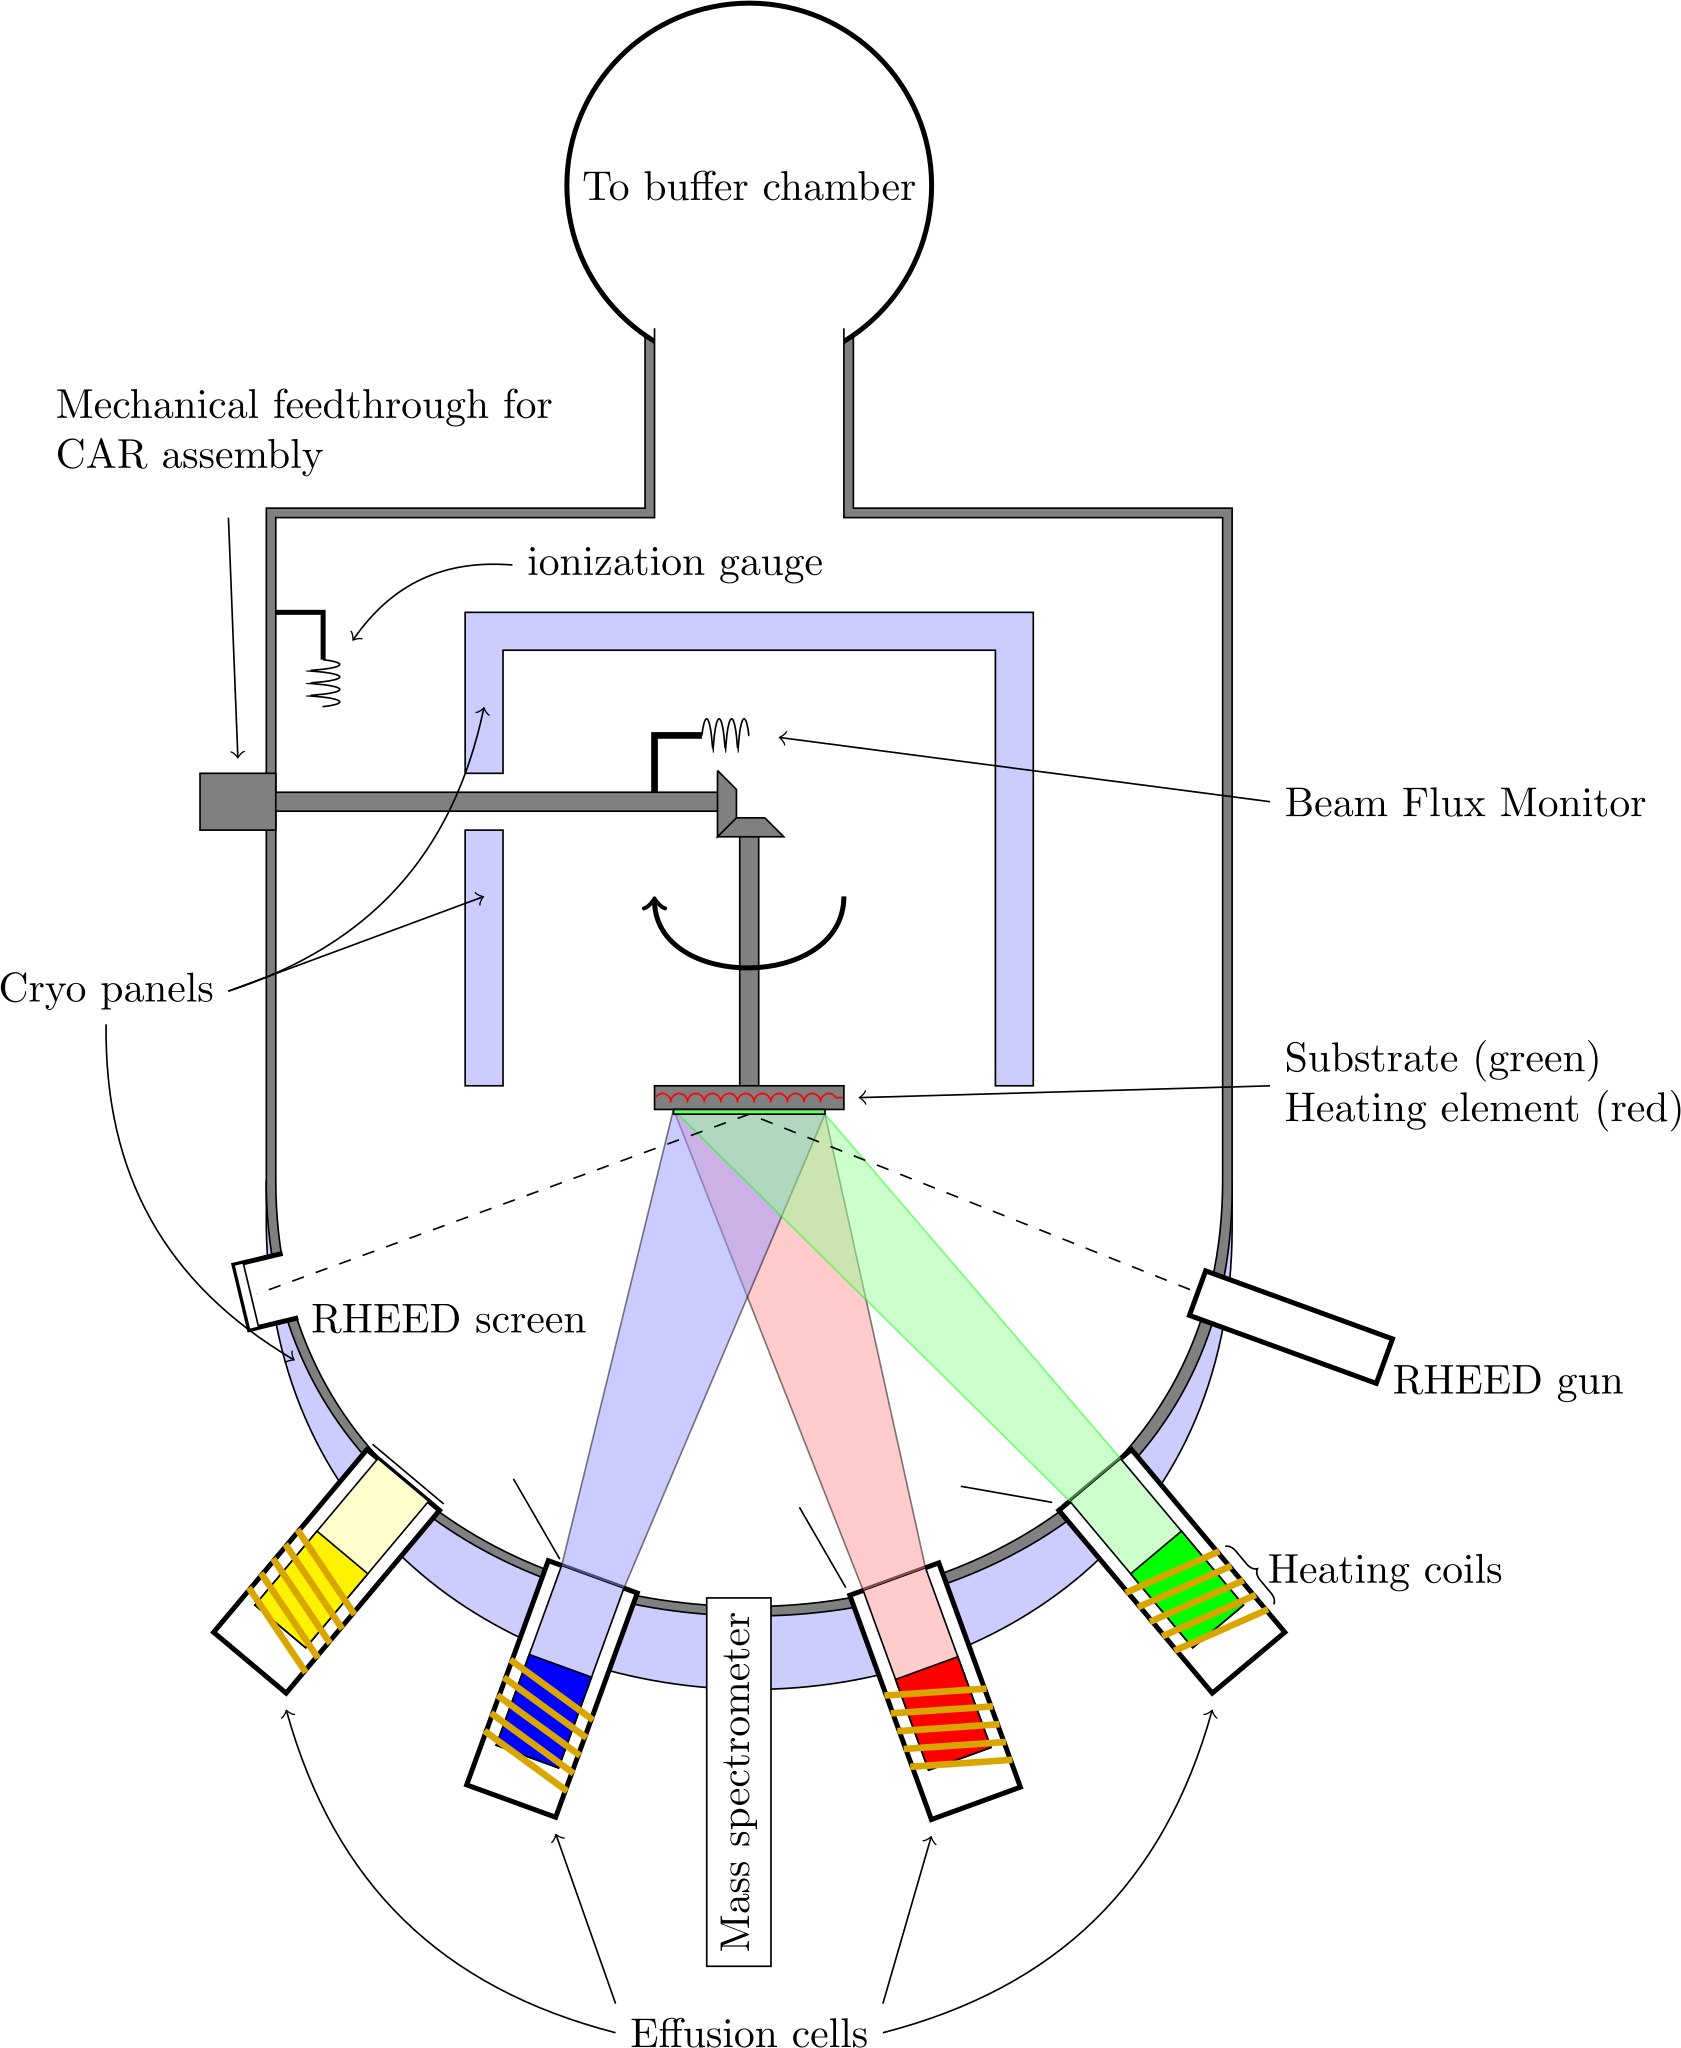
\includegraphics[scale = 0.5]{MBE.png}
        \caption{\tiny{MBE apparatus}\\ \tiny{By Vegar Ottesen - Own work https//:commons.wikimedia.org/w/index.php?curid=16957521}}
        \label{MBE apparatus}
    \end{figure}
\end{frame}


\begin{frame}{Electron Beam Lithography}
    \begin{figure}
        \centering
        \begin{subfigure}
            \includegraphics[scale = 0.15]{EBL1.png}
            \label{EBL1}
        \end{subfigure}
        \hfill
        \begin{subfigure}
            \includegraphics[scale = 0.15]{EBL2.png}
            \label{EBL2}
        \end{subfigure}
        \hfill
        \begin{subfigure}
            \includegraphics[scale = 0.15]{EBL3.png}
            \label{EBL3}
        \end{subfigure}

        \begin{subfigure}
            \includegraphics[scale = 0.15]{EBL4.png}
            \label{EBL4}
        \end{subfigure}
        \hfill
        \begin{subfigure}
            \includegraphics[scale = 0.15]{EBL5.png}
            \label{EBL5}
        \end{subfigure}
        \hfill
        \begin{subfigure}
            \includegraphics[scale = 0.15]{EBL6.png}
            \label{EBL6}
        \end{subfigure}
        \caption{\tiny{Building in Zero Dimensions from Quantum Dots by Mark A. Reed}}
    \end{figure}
\end{frame}


% \begin{frame}{Electric Gating}
%     \begin{itemize}
%     \item uses MBE (in Frank–van der Merwe mode) to grow the Doped Semiconducting layer (e.g. AlGaAs) over an undoped substrate (e.g. GaAs).
%     \item Uses EBL to grow nano-electrodes on the substrate.
%     \item By controlling the applied voltage to the nano-electrode, potential barriers form, and the electrons are confined.
%     \item Easier control over size and shape.
%     \end{itemize}
%     \begin{wrapfigure}{l}{0.5\textwidth}
%         \begin{figure}
%             \begin{subfigure}
%                 \includegraphics[scale = 0.15]{E_Gating.png}
%             \end{subfigure}

%             \begin{subfigure}
%                 \includegraphics[scale = 0.15]{E_Gating.png}
%             \end{subfigure}

            
%             \caption{\tiny{from Quantum Dots by Mark A. Reed}}
%             \label{Egating and SET}
%         \end{figure}
%     \end{wrapfigure}
% \end{frame}


\begin{frame}{Electric Gating}
    \begin{columns}
        \begin{column}{0.6\textwidth}
            \begin{itemize}
                \item Uses MBE (in Frank–van der Merwe mode) to grow the doped semiconducting layer (e.g. AlGaAs) over an undoped substrate (e.g. GaAs).
                \item Uses EBL to grow nano-electrodes on the substrate.
                \item By controlling the applied voltage to the nano-electrode, potential barriers form, and the electrons are confined.
                \item Easier control over size and shape.
                \item SET.
            \end{itemize}
        \end{column}

        \begin{column}{0.4\textwidth}
            \begin{figure}
                \centering
                \begin{subfigure}
                    \includegraphics[scale = 0.15]{E_Gating.png}(a)
                \end{subfigure}

                \begin{subfigure}
                    \includegraphics[scale = 0.15]{SET.png}(b)
                \end{subfigure}
                \caption{\Tiny{(a) from Quantum Dots by Mark A. Reed. (b) SET from Statistics and Parametric Correlations of Coulomb Blockade Peak Fluctuations in Quantum Dots by J. A. Folk(1996)}}
                \label{Egating and SET}
            \end{figure}
        \end{column}
    \end{columns}
\end{frame}


\begin{frame}{Electric Gating}{Single Electron Transistor}
    \begin{columns}
        \begin{column}{0.6\textwidth}
            \begin{itemize}
                \item Under certain tunneling conditions, electrons from adjacent 2D electron reservoirs can tunnel through the quantum dot.
                \item  tunneling is blocked by the Coulomb blockade.
                \item  if the energy of the dot decrease and a potential difference is introduced between both reservoirs (call them drain and source) such that $ \mu_d< E_{N+1} < \mu_s$ then current will flow from the source to the drain.
            \end{itemize}
        \end{column}

        \begin{column}{0.4\textwidth}
            \begin{figure}
                \centering
                \begin{subfigure}
                    \includegraphics[scale = 0.15]{SET2.png}(a)
                \end{subfigure}

                \begin{subfigure}
                    \includegraphics[scale = 0.20]{Coloumb Blockade.png}(b)
                \end{subfigure}
                \caption{\Tiny{(a) SET from Statistics and Parametric Correlations of Coulomb Blockade Peak Fluctuations in Quantum Dots by J. A. Folk(1996). (b) Coulomb Blockade (Kittel)}}
                \label{Egating and SET}
            \end{figure}
        \end{column}
    \end{columns}
\end{frame}


\begin{frame}{Energy Calculation}{Simple QW model}
    \begin{itemize}
        \item Quantum dots are usually modeled as 3D quantum wells.
        \item Spherical Finite and infinite wells have shown high accuracy for measuring the transition energies of spherical quantum dots with errors smaller than $3\%$ in the energy value.
        \[ E_{n,l} = \frac{\hbar^2 \beta^2 n,l^2}{2 m_{\text{eff}} R^2} \]
        \item this model shows that Energy levels confinement goes down as $\Delta E \propto 1/R^2$
    \end{itemize}
\end{frame}

\begin{frame}{Energy Calculation}{Simple QW model}
    \begin{itemize}
        \item Quantum dots are not restricted to spherical shapes. Based on the growth process different more complicated shapes are possible.
        \item Here I will tackle a case of InAs Quantum dot. Where the Stranki-Krastanov results in a conic shape of the dot.
        \item The dot is assumed to have a perfect conic shape with a small elevation angle of $\pi/15$.
        \item The transition energies were solved for holes and electrons. by numerically solving the Schrodinger Equation.
        \item The parameters were obtained from J.Y. Marzin paper.
    \end{itemize}
\end{frame}

\begin{frame}{Numerical Solution}
    \begin{itemize}
        \item Discretization of space, and vectorization of the $2D$ $(N\times M)$ grid to $NM$-dimensional vector.
        \begin{figure}
            \centering
            \includegraphics[scale=0.3]{Vectorization.jpg}
            \label{fig:discretization}
        \end{figure}
    \end{itemize}
\end{frame}



\begin{frame}{Numerical Solution}
    \begin{itemize}
        \item Due to Azimuthal symmetry we can write the Hamiltonian as:
        \begin{equation}
            \mathcal{H}(r, z) = -\frac{\hbar^2}{2}\left( \frac{1}{m}\frac{\partial^2}{\partial z^2} + \frac{1}{m}\frac{1}{r}\frac{\partial}{\partial r} r \frac{\partial}{\partial r}\right) - \frac{n^2}{m r^2} + \mathrm{V}(r, z) 
            \label{Hamiltonian}
        \end{equation}

        \item redefine $r = r/R$ and $z = z/Z$ so that $r, z$ are dimensionless where $R, Z$ are big enough to be considered infinite (in this scenario, I chose $Z = R = 40nm$)

        \item Under these transformations, the Hamiltonian can be written in a matrix form as:
        \begin{equation}
            \begin{split}
            H^i_k = & \frac{-\hbar^2}{2mR^2}\left( \frac{ \delta^{i-1}_k -2 \delta^{i}_k + \delta^{i+1}_k} {\Delta r^2} + \frac{\delta^{i-1}_k - \delta^{i+1}_k}{2r_i\Delta r} - \frac{n^2}{r_i^2}\delta^{i}_k\right) \\
            & + \frac{-\hbar^2}{2mZ^2}\left(\frac{\delta^{i-N}_k -2\delta^{i}_k + \delta^{i+N}_k}{\Delta z^2}\right) + V^i \delta^i_k
            \end{split}
            \label{H matrix}
        \end{equation}
    \end{itemize}
\end{frame}

\begin{frame}{Numerical Solution}
    \begin{itemize}
        \item The discretization length I took was $N = M = 128$, $NM = 16384$.
        \item The aforementioned Hamiltonian is a sparse matrix, therefore I used \textbf{scipy.sparse} python library to solve for its eigenvalues.
        \item Boundary Conditions:
        \begin{itemize}
            \item $\psi(r \to \infty, z, \phi) = \psi(r, z \to \pm\infty, 0) = 0$
            \item $\left.\frac{\partial}{\partial r}\psi(r, z, \phi)\right|_{r\to 0} = 0$
            \item The first condition is satisfied be default with the definition of the matrix
            \item The second condition is achieved by defining modifying the derivative matrices as follows:
            \begin{align}
                \partial^2_r [0, 0]_{(r=0)} =& -1\\
                \partial_r [0, 1] =& 0
            \end{align}
        \end{itemize}
    \end{itemize}
\end{frame}


\begin{frame}{Result}
\begin{figure}
    \centering
    \begin{subfigure}
        \includegraphics[scale = 0.25]{Qdot1ML.png}(a)&
    \end{subfigure}
    \begin{subfigure}
        \includegraphics[scale = 0.25]{Tenergies.png}(b)
    \end{subfigure}
    \begin{subfigure}
        \includegraphics[scale = 0.22]{Paper_energies.png}(c)&
    \end{subfigure}
    \begin{subfigure}
        \includegraphics[scale = 0.17]{paper_Transitions.png}(d)
    \end{subfigure}
    \caption{Results for solving for the state energies and transition energies in InAs/GaAs QD. The paper's results are included for comparison, the paper reported that the average transition energy of InAs/GaAs QD at $R = 13.5nm$ is $1.07eV$ while it was found using my code to be $1.0677$ eV}
    \label{fig: results}
\end{figure}
    
\end{frame}



\begin{frame}{Energy Dependence in Effective Mass}
    \begin{columns}
        \begin{column}{0.4\textwidth}
            \begin{itemize}
            \item Correction by introducing energy dependence in effective mass term.
            \item Iterative non-linear scheme used for solving.
            \item Effective mass recalculated with updated energy values until convergence.
            \end{itemize}

            \Small\begin{equation}
                \begin{split}
                    \frac{1}{m(E)} &\propto \left( \frac{2}{E + E_g - V} \\&+ \frac{1}{E + E_g + \Delta - V} \right)
                \end{split}
                
                \label{effictive mass}
            \end{equation}
        \end{column}

        \begin{column}{0.60\textwidth}
            \begin{figure}[t]
                \centering
                \includegraphics[scale=0.35]{iterative.jpg}
                \caption{Iterative scheme for solving non-linear eigenvalue problems}
                \label{fig:iterative}
            \end{figure}
        \end{column}
    \end{columns}
    
\end{frame}


\begin{frame}{Density Functional Theory (DFT)}{limitations of Simple models}
    \begin{itemize}
        \item As the size of the dot gets smaller surface area to volume ratio increase.
        \item As a result, surface defects (legends, additional atoms, or missing atoms) will have high impact on the energy levels. 
        \item smooth surfaces approximation are no longer be valid. And Incorporating such changes will require finer discretizations.
        \item More suffocated methods and approximations can provide a better understanding of the behaviour and solution. One of these methods is the DFT.
        \item Useful for studying the Coulomb blockade related effects, such as the peak spacing in the conductance through the dot
    \end{itemize}
\end{frame}


\begin{frame}{Kohn-Sham Hamiltonian and Energy Functional}
	\framesubtitle{Kohn-Sham Hamiltonian}
	\[
	\hat{H}^\sigma = -\frac{1}{2} \nabla^2 + V^\sigma_{\text{ext}}(\mathbf{r}) + V^\sigma_{\text{H}}(\mathbf{r}) + V^\sigma_{\text{XC}}(\mathbf{r})
	\]
	\begin{itemize}
		\item \textbf{Spin}: $\sigma \in \{\alpha, \beta\}$
		\item \textbf{Exchange-Correlation Potential}: $V_{\text{XC}}$ - purely quantum term from fermions' anti-symmetric behavior.
		\item \textbf{Hartree Potential}: $E\int \frac{n(\mathbf{r})}{|\mathbf{r} - \mathbf{r'}|} \, d\mathbf{r}$
	\end{itemize}
	\framesubtitle{Energy Functional}
	\[
	\begin{aligned}
		E[n^\alpha(\mathbf{r}), n^\beta(\mathbf{r})] &= T[n^\alpha(\mathbf{r}), n^\beta(\mathbf{r})] + \int_{\mathbf{r}} n(\mathbf{r}) V_{\text{ext}}(\mathbf{r}) \, d\mathbf{r} \\
		&\quad + \int_{\mathbf{r}}\int_{\mathbf{r'}} \frac{n(\mathbf{r})n(\mathbf{r'})}{|\mathbf{r} - \mathbf{r'}|}\, d\mathbf{r} d\mathbf{r'} + E_{\text{XC}}[n^\alpha(\mathbf{r}), n^\beta(\mathbf{r})]
	\end{aligned}
	\]
	\begin{itemize}
		\item \textbf{Density of Spin Orbitals}: $n^\sigma(\mathbf{r}) = \sum_i^{N^\alpha} |\psi^\sigma_i(\mathbf{r})|^2$
	\end{itemize}
\end{frame}

\begin{frame}{Kinetic Energy and Iterative Scheme}
	\framesubtitle{Kinetic Energy}
	\[
	T[n^\alpha(\mathbf{r}), n^\beta(\mathbf{r})] = -\frac{1}{2}\sum_{i, \sigma} \langle \psi_i^\sigma | \nabla^2 | \psi_i^\sigma \rangle
	\]
	\begin{itemize}
		\item \textbf{Single Electron States}: $\{\psi_i^\sigma(\mathbf{r})\}$
	\end{itemize}
	\framesubtitle{Solving Single Orbital States}
	\[
	\hat{H}^\sigma|\psi_i^\sigma(\mathbf{r})\rangle = \epsilon_i^\sigma |\psi_i^\sigma(\mathbf{r})\rangle
	\]
	\begin{itemize}
		\item \textbf{Iterative Scheme}:
		\begin{itemize}
			\item Assume trial functions $\{\psi_i^\sigma(\mathbf{r})\}$
			\item Find $\{n^\alpha(\mathbf{r}), n^\beta(\mathbf{r})\}$
			\item Calculate $E[n^\alpha(\mathbf{r}), n^\beta(\mathbf{r})]$
			\item Check for convergence based on energy values
			\item Solve for $\{\psi^\prime_i^\sigma(\mathbf{r})\}$
			
		\end{itemize}
	\end{itemize}
	\framesubtitle{Exchange-Correlation Energy Approximations}
	\item \textbf{Drawbacks}: No exact method to calculate $E_{\text{XC}}$, therefore Spin-polarized uniform electron gas is used to approximate  $E_{\text{XC}}$ (local-spin-density approximation (\textbf{LSDA})).
	
\end{frame}


\begin{frame}{Experimental Results: PL and PLE}
    \begin{columns}
        \begin{column}{0.6\textwidth}
            \begin{itemize}
                \item Electromagnetic radiation emission from any form of matter after the absorption of photons. In PL the absorbed photon is applied and the emitted photons are observed, in case of PLE the opposite is being done.
                \item Sensitive to phonon emissions, as excited electron may not relax directly to ground state, with relaxation efficiency that depends on energy.
                \item excited-state energies cannot be determined directly from the spectra.
            \end{itemize}
        \end{column}
        \begin{column}{0.4\textwidth}
            \begin{figure}
                \centering
                \includegraphics[scale=0.4]{PLE.png}
                \label{fig:PLE}
            \end{figure}
        \end{column}
    \end{columns}
\end{frame}


\begin{frame}{CV Analysis of Quantum Dots}
    \begin{columns}
        \begin{column}{0.6\textwidth}
            \begin{itemize}
                \item CV test can analyze the energy gap of Quantum dots.
                \item Hole energy at the top of the valence band and electron energy at the edge of the conduction band are proportional to respective cathodic and anodic peaks in the CVs.
                \item The voltage difference directly correlates to the dot's band gap.
                \item As the Q-dot size decreases, the cathodic and anodic peaks shift to higher energies, increasing the gap energy.
                
            \end{itemize}
        \end{column}
        \begin{column}{0.4\textwidth}
            \begin{figure}
                \centering
                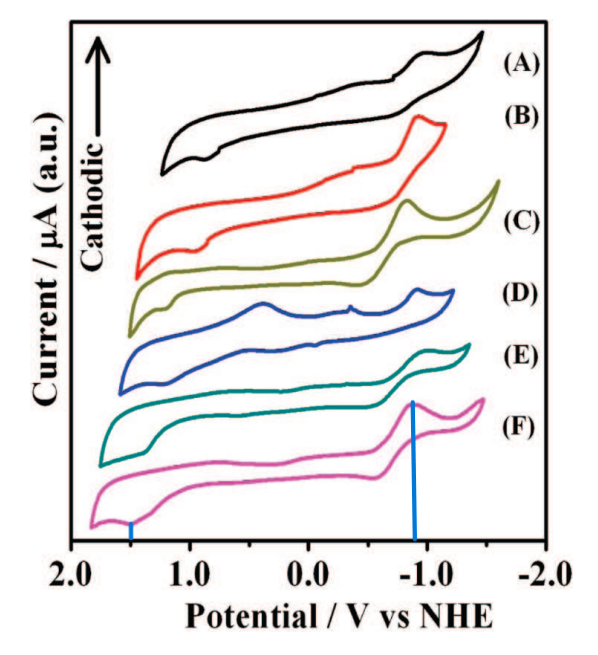
\includegraphics[scale=0.3]{CV_QDs.png}
                \caption{CV Spectrum for Different QD Sizes}
                \label{fig:CV}
            \end{figure}
        \end{column}
    \end{columns}
\end{frame}


\begin{frame}{Energy tuning}{Growth Temperature}
    \begin{itemize}
        \item The shell structure can be tuned by adjusting the substrate temperature during the formation of the QDs.
        \item Larger QDs with smaller band gap energies are obtained at higher growth temperatures.
        \item The intermixing between QDs is reduced when the growth temperature is lowered, increasing the uniformity of the QDs.
    \end{itemize}
\end{frame}

\begin{frame}{Energy tuning}{QD Density}
    \begin{columns}
        \begin{column}{0.65\textwidth}
            \begin{itemize}
                \item To obtain uniform QDs with well-defined energy levels, the QD density must be kept low.
                \item Stranski-Krastanow growth mode for InAs/GaAs occurs at about 1.6 ML (And higher).
                \item For denser coverages, wave function states from neighboring dots starts to overlap.
            \end{itemize}
        \end{column}
        \begin{column}{0.40\textwidth}
            \begin{figure}
                \centering
                \includegraphics[scale = 0.4]{coverage.png}
                \label{fig:In coverage}
            \end{figure}
        \end{column}

    \end{columns}
\end{frame}

\begin{frame}{Energy tuning}{Thermal Annealing}
    \begin{columns}
        \begin{column}{0.65\textwidth}
            \begin{itemize}
                \item Tuning of the QD interband transition energy can be achieved using rapid thermal annealing (RTA).
                \item RTA has the effects of blue-shift, narrowing PL line-width, and decreasing intersublevel spacing energies as the annealing temperature increases.
                \item TEM images show that the QD size does not change significantly with RTA.
                \item Changes in energy levels are attributed to the increase of Ga concentration in QDs due to the inter-diffusion of In–Ga atoms at the interface between the QD and the GaAs barrier.
            \end{itemize}
        \end{column}
        \begin{column}{0.5\textwidth}
            \begin{figure}
                \centering
                \includegraphics[scale=0.4]{PL annealing.png}
                \label{fig:annealing}
            \end{figure}
        \end{column}
    \end{columns}
\end{frame}


\begin{frame}{Graphene Quantum Dots}
    \begin{itemize}
        \item As expected, the energy gap decreases as the size of the GQD increases, however, with some types of GQDs, the proportionality is $\Delta E \propto 1/L$ which is different from the conventional case, and marks the possibility to produce bigger quantum dots where confinement is still possible.
        \item Whether GCDs have been experimentally made is still a matter of dispute, some papers claim that they have successfully made GCDs at laboratories, others argue that are these are rather fluorescent organic dots
    \end{itemize}
    
\end{frame}




% \addbibresource{references.bib}

% \usepackage{biblatex}
\bibliographystyle{plain}
\bibliography{references}
\section{References}
    \nocite{reed1993quantum}
    \nocite{shur1989gallium}
    \nocite{hsu2000tuning}
    \nocite{alhassid2000statistical}
    \nocite{pu2018colloidal}
    \nocite{marzin1994calculation}
    \nocite{li2001computer}
    \nocite{sDFT}
    \nocite{10.1063/1.3284083}
    \nocite{kilina2016surface}
    \nocite{haram2011quantum}
    \nocite{steer1996electronic}
    \nocite{fafard1999manipulating}
    \nocite{zhang2008tuning}
    \nocite{silvestrov2007quantum}
% \begin{frame}[noframenumbering,plain,allowframebreaks]
%     \nocite{reed1993quantum}
%     \nocite{shur1989gallium}
%     \nocite{hsu2000tuning}
%     \nocite{alhassid2000statistical}
%     \nocite{pu2018colloidal}
%     \nocite{marzin1994calculation}
%     \nocite{li2001computer}
%     \nocite{sDFT}
%     \nocite{10.1063/1.3284083}
%     \nocite{kilina2016surface}
%     \nocite{haram2011quantum}
%     \nocite{steer1996electronic}
%     \nocite{fafard1999manipulating}
%     \nocite{zhang2008tuning}
%     \nocite{silvestrov2007quantum}
%     % \printbibliography[heading=none]
% \end{frame}


% \begin{frame}%{References (1/3)}
    
%     \nocite{reed1993quantum}
%     \nocite{shur1989gallium}
%     \nocite{hsu2000tuning}
%     \nocite{alhassid2000statistical}
%     \nocite{pu2018colloidal}
% % \end{frame}
% % \begin{frame}{References (2/3)}
   
%     \nocite{marzin1994calculation}
%     \nocite{li2001computer}
%     \nocite{sDFT}
%     \nocite{10.1063/1.3284083}
%     \nocite{kilina2016surface}
%     \nocite{haram2011quantum}
% % \end{frame}
% % \begin{frame}{References (3/3)}

%     \nocite{steer1996electronic}
%     \nocite{fafard1999manipulating}
%     \nocite{zhang2008tuning}
%     \nocite{silvestrov2007quantum}
%     % \printbibliography
% \end{frame}


\end{document}